\documentclass[tikz,border=0]{standalone}
\usepackage[T1]{fontenc}
\usepackage[utf8]{inputenc}
\usepackage[defaultfam,light,semibold,bold]{montserrat}
\renewcommand{\familydefault}{\sfdefault}
\newcommand{\MBold}{\fontseries{b}\selectfont}
\newcommand{\MLight}{\fontseries{l}\selectfont}
\usepackage{graphicx}
\usepackage{xcolor}
\usepackage{tikz}

\graphicspath{{figures/}}

\definecolor{paper}{HTML}{D8DDE3}
\definecolor{ink}{HTML}{1C2229}
\definecolor{card}{HTML}{FFFFFF}
\definecolor{accent}{HTML}{1F6FBF}
\definecolor{ok}{HTML}{1F8A4C}
\definecolor{bad}{HTML}{C7353B}
\definecolor{muted}{HTML}{5C6670}

\begin{document}
\begin{tikzpicture}[every node/.style={inner sep=0,outer sep=0}]

\fill[paper] (0,0) rectangle (420mm,594mm);
\fill[accent] (0,0) rectangle (8mm,594mm);

% ===== HEADLINE ============================================================
\node[anchor=north west,text=accent,font=\MBold]
  at (22mm,584mm) {\fontsize{15}{18}\selectfont PYPLANT};
\node[anchor=north east,text=muted,font=\MLight]
  at (400mm,584mm)
  {\fontsize{10}{13}\selectfont TWO-TANK PROCESS \,$\cdot$\, SOFT PLC \,$\cdot$\, SCADA \,$\cdot$\, FAULT DIAGNOSIS};

\node[anchor=north west,text=ink,font=\MBold]
  at (22mm,560mm) {\fontsize{54}{60}\selectfont Break the plant.};
\node[anchor=north west,text=ink,font=\MBold]
  at (22mm,530mm) {\fontsize{54}{60}\selectfont Watch who notices.};

\node[anchor=north west,text=muted,align=left,text width=190mm,
  font=\MLight]
  at (22mm,498mm)
  {\fontsize{15}{21}\selectfont
   A live two-tank unit with its PID, PLC, historian and operator HMI ---
   and four detectors that compete to find a leak the alarms never see.};

\foreach \i/\lab/\col in {
  0/{1 \, scenario}/accent, 1/{2 \, live stack}/accent,
  2/{3 \, inject leak}/bad, 3/{4 \, dataset}/accent,
  4/{5 \, train}/ok, 5/{6 \, stop}/ink}
{
  \fill[\col,rounded corners=3pt] ({22mm+\i*31mm},444mm) rectangle ({51mm+\i*31mm},464mm);
  \node[anchor=center,text=white,font=\MBold]
    at ({36.5mm+\i*31mm},454mm) {\fontsize{10}{12}\selectfont \lab};
}

% hero screenshot
\fill[ink!15] (220mm,330mm) rectangle (402mm,486mm);
\fill[card] (218mm,332mm) rectangle (400mm,488mm);
\node[anchor=center] at (309mm,410mm)
  {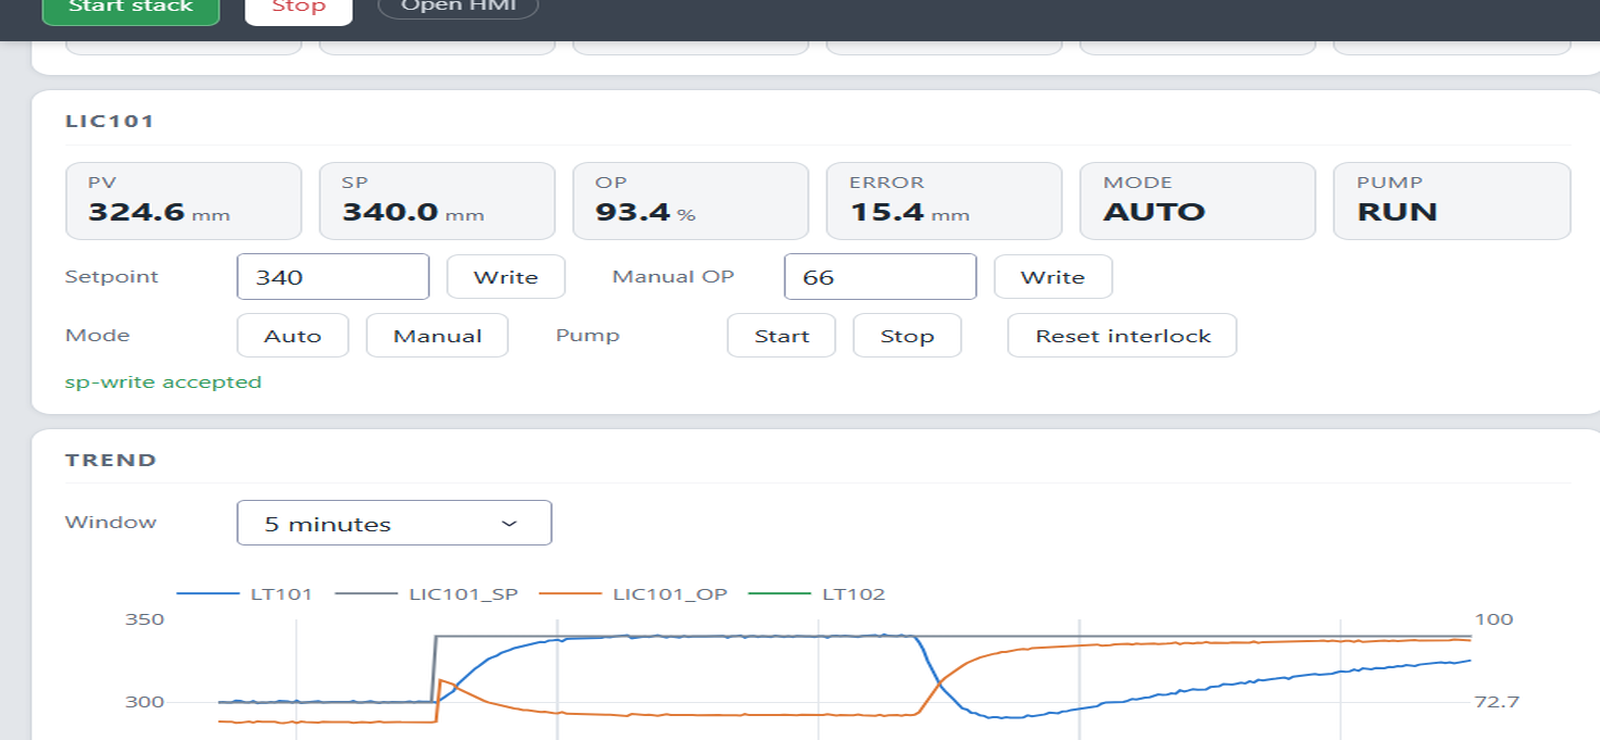
\includegraphics[width=174mm]{poster_hero}};
\node[anchor=north east,text=muted,font=\MLight]
  at (400mm,326mm)
  {\fontsize{10}{13}\selectfont Runtime \,$\cdot$\, leak in tank 1 \,$\cdot$\, OP 93\%, no alarm};

% ===== THREE PRODUCT SHOTS =================================================
\foreach \x/\file/\cap in {
  22mm/poster_mimic/{The plant. Tank 1 at 300 mm, valve at 66\%.},
  148mm/poster_hmi/{The operator HMI. Mimic, live trend, ISA-18.2 alarms.},
  274mm/poster_model/{Trained detectors. PCA selected: 88\%, 0 false alarms/day.}}
{
  \fill[ink!15] ({\x+1.5mm},202mm) rectangle ({\x+125.5mm},318mm);
  \fill[card] (\x,204mm) rectangle ({\x+124mm},320mm);
  \node[anchor=north] at ({\x+62mm},318mm)
    {\includegraphics[width=120mm]{\file}};
  \node[anchor=north west,text=muted,align=left,text width=122mm,
    font=\MLight]
    at (\x,198mm) {\fontsize{11}{15}\selectfont \cap};
}

% ===== FEATURE CARDS =======================================================
\fill[card] (22mm,72mm) rectangle (146mm,184mm);
\fill[ok] (22mm,180mm) rectangle (146mm,184mm);
\node[anchor=north west,text=ink,font=\MBold]
  at (30mm,172mm) {\fontsize{17}{21}\selectfont Live stack};
\node[anchor=north west,text=muted,align=left,text width=106mm,
  font=\MLight]
  at (30mm,150mm)
  {\fontsize{11}{15}\selectfont
   Plant, PLC, historian and HMI. Start, stop and speed them. Operate LIC101. Inject a leak. Watch the loop hide it.};
\node[anchor=north west,text=ink,align=left,font=\MLight]
  at (30mm,112mm)
  {\fontsize{10}{14}\selectfont
   \begin{tabular}{@{}p{26mm}l@{}}
   plant & Modbus 5400\\
   PLC & scan 100 ms, OPC UA 5403\\
   historian & DuckDB, LOCF windows\\
   HMI & mimic, trend, ISA-18.2
   \end{tabular}};

\fill[card] (150mm,72mm) rectangle (274mm,184mm);
\fill[bad] (150mm,180mm) rectangle (274mm,184mm);
\node[anchor=north west,text=ink,font=\MBold]
  at (158mm,172mm) {\fontsize{17}{21}\selectfont Break something};
\node[anchor=north west,text=muted,align=left,text width=106mm,
  font=\MLight]
  at (158mm,150mm)
  {\fontsize{11}{15}\selectfont
   Leak, stiction, worn pump, fouling, a lying sensor. Nobody is told. The only way to know is to watch the plant.};
\node[anchor=north west,text=ink,align=left,font=\MLight]
  at (158mm,112mm)
  {\fontsize{10}{14}\selectfont
   \begin{tabular}{@{}p{30mm}l@{}}
   Leak in tank 1 & OP rises 25 points\\
   Sticking valve & ZT lags OP in steps\\
   Worn pump & PT and FT drop\\
   Sensor bias & ground truth disagrees
   \end{tabular}};

\fill[card] (278mm,72mm) rectangle (400mm,184mm);
\fill[accent] (278mm,180mm) rectangle (400mm,184mm);
\node[anchor=north west,text=ink,font=\MBold]
  at (286mm,172mm) {\fontsize{17}{21}\selectfont Train. Compare. Deploy.};
\node[anchor=north west,text=muted,align=left,text width=104mm,
  font=\MLight]
  at (286mm,150mm)
  {\fontsize{11}{15}\selectfont
   Z-score, PCA, isolation forest, autoencoder. Best detection wins; ties go to the simpler method.};
\node[anchor=north west,text=ink,align=left,font=\MLight]
  at (286mm,112mm)
  {\fontsize{10}{14}\selectfont
   \begin{tabular}{@{}p{32mm}l@{}}
   PCA (selected) & 88\% detected, 43 s\\
   Autoencoder & 88\%, later isolation\\
   Z-score & 62\%, 341 s\\
   Isolation forest & 38\%
   \end{tabular}};

% ===== NUMBERS =============================================================
\foreach \x/\n/\l in {
  70mm/4/{live services}, 162mm/7/{fault modes},
  254mm/4/{detectors}, 346mm/0/{alarms on the leak}}
{
  \node[anchor=center,text=ink,font=\MBold]
    at (\x,54mm) {\fontsize{34}{38}\selectfont \n};
  \node[anchor=center,text=muted,font=\MLight]
    at (\x,36mm) {\fontsize{12}{15}\selectfont \l};
}

% ===== FOOTER ==============================================================
\fill[ink] (0,0) rectangle (420mm,18mm);
\node[anchor=west,text=white,font=\MLight]
  at (22mm,9mm)
  {\fontsize{10}{13}\selectfont
   conda activate pyplant \quad python -m pyplant.workbench.app --workspace ./work/manual \quad then open  http://127.0.0.1:8050};
\node[anchor=east,text=white,font=\MLight]
  at (398mm,9mm)
  {\fontsize{10}{13}\selectfont quickguide.pdf \,$\cdot$\, main.pdf \,$\cdot$\, walkthrough.mp4};

\end{tikzpicture}
\end{document}
